\chapter[Design af mekanik]{Mekanik}
\mnote{Nick Østergaard og Christian Klim Hansen}

% Her beskrives de overvejelser vi har haft omkring udformningen af
% vores mekanik.

I vores overvejeler omkring udformningen af vores produkt, så vi på
selve funktionen af produktet. Fordi vores produktet har til formål at
plotte en figur på et stykke A4-papir, så er det vigtigt, at
mekanikken er så slørfri som muligt. For at undgå slør har vi set på
placeringen af pennen, forskellige konstruktioner til akserne, og
hvilken metode vi vil bruge til at flytte akserne med.

Vi havde to forskellige forslag til udformningen glideren. De to
stænger, som pennen kører på, kunne enten være placeret vandret, som
ses på figur\vref{fig:glider}, eller lodret. Vi kom frem
til, at det, som ville resultere i mindst slør, var, hvis gliderne var
placeret vandret. Pennen styres af en stepmotor, som er placeret ude i
en af siderne.

\mnote{
  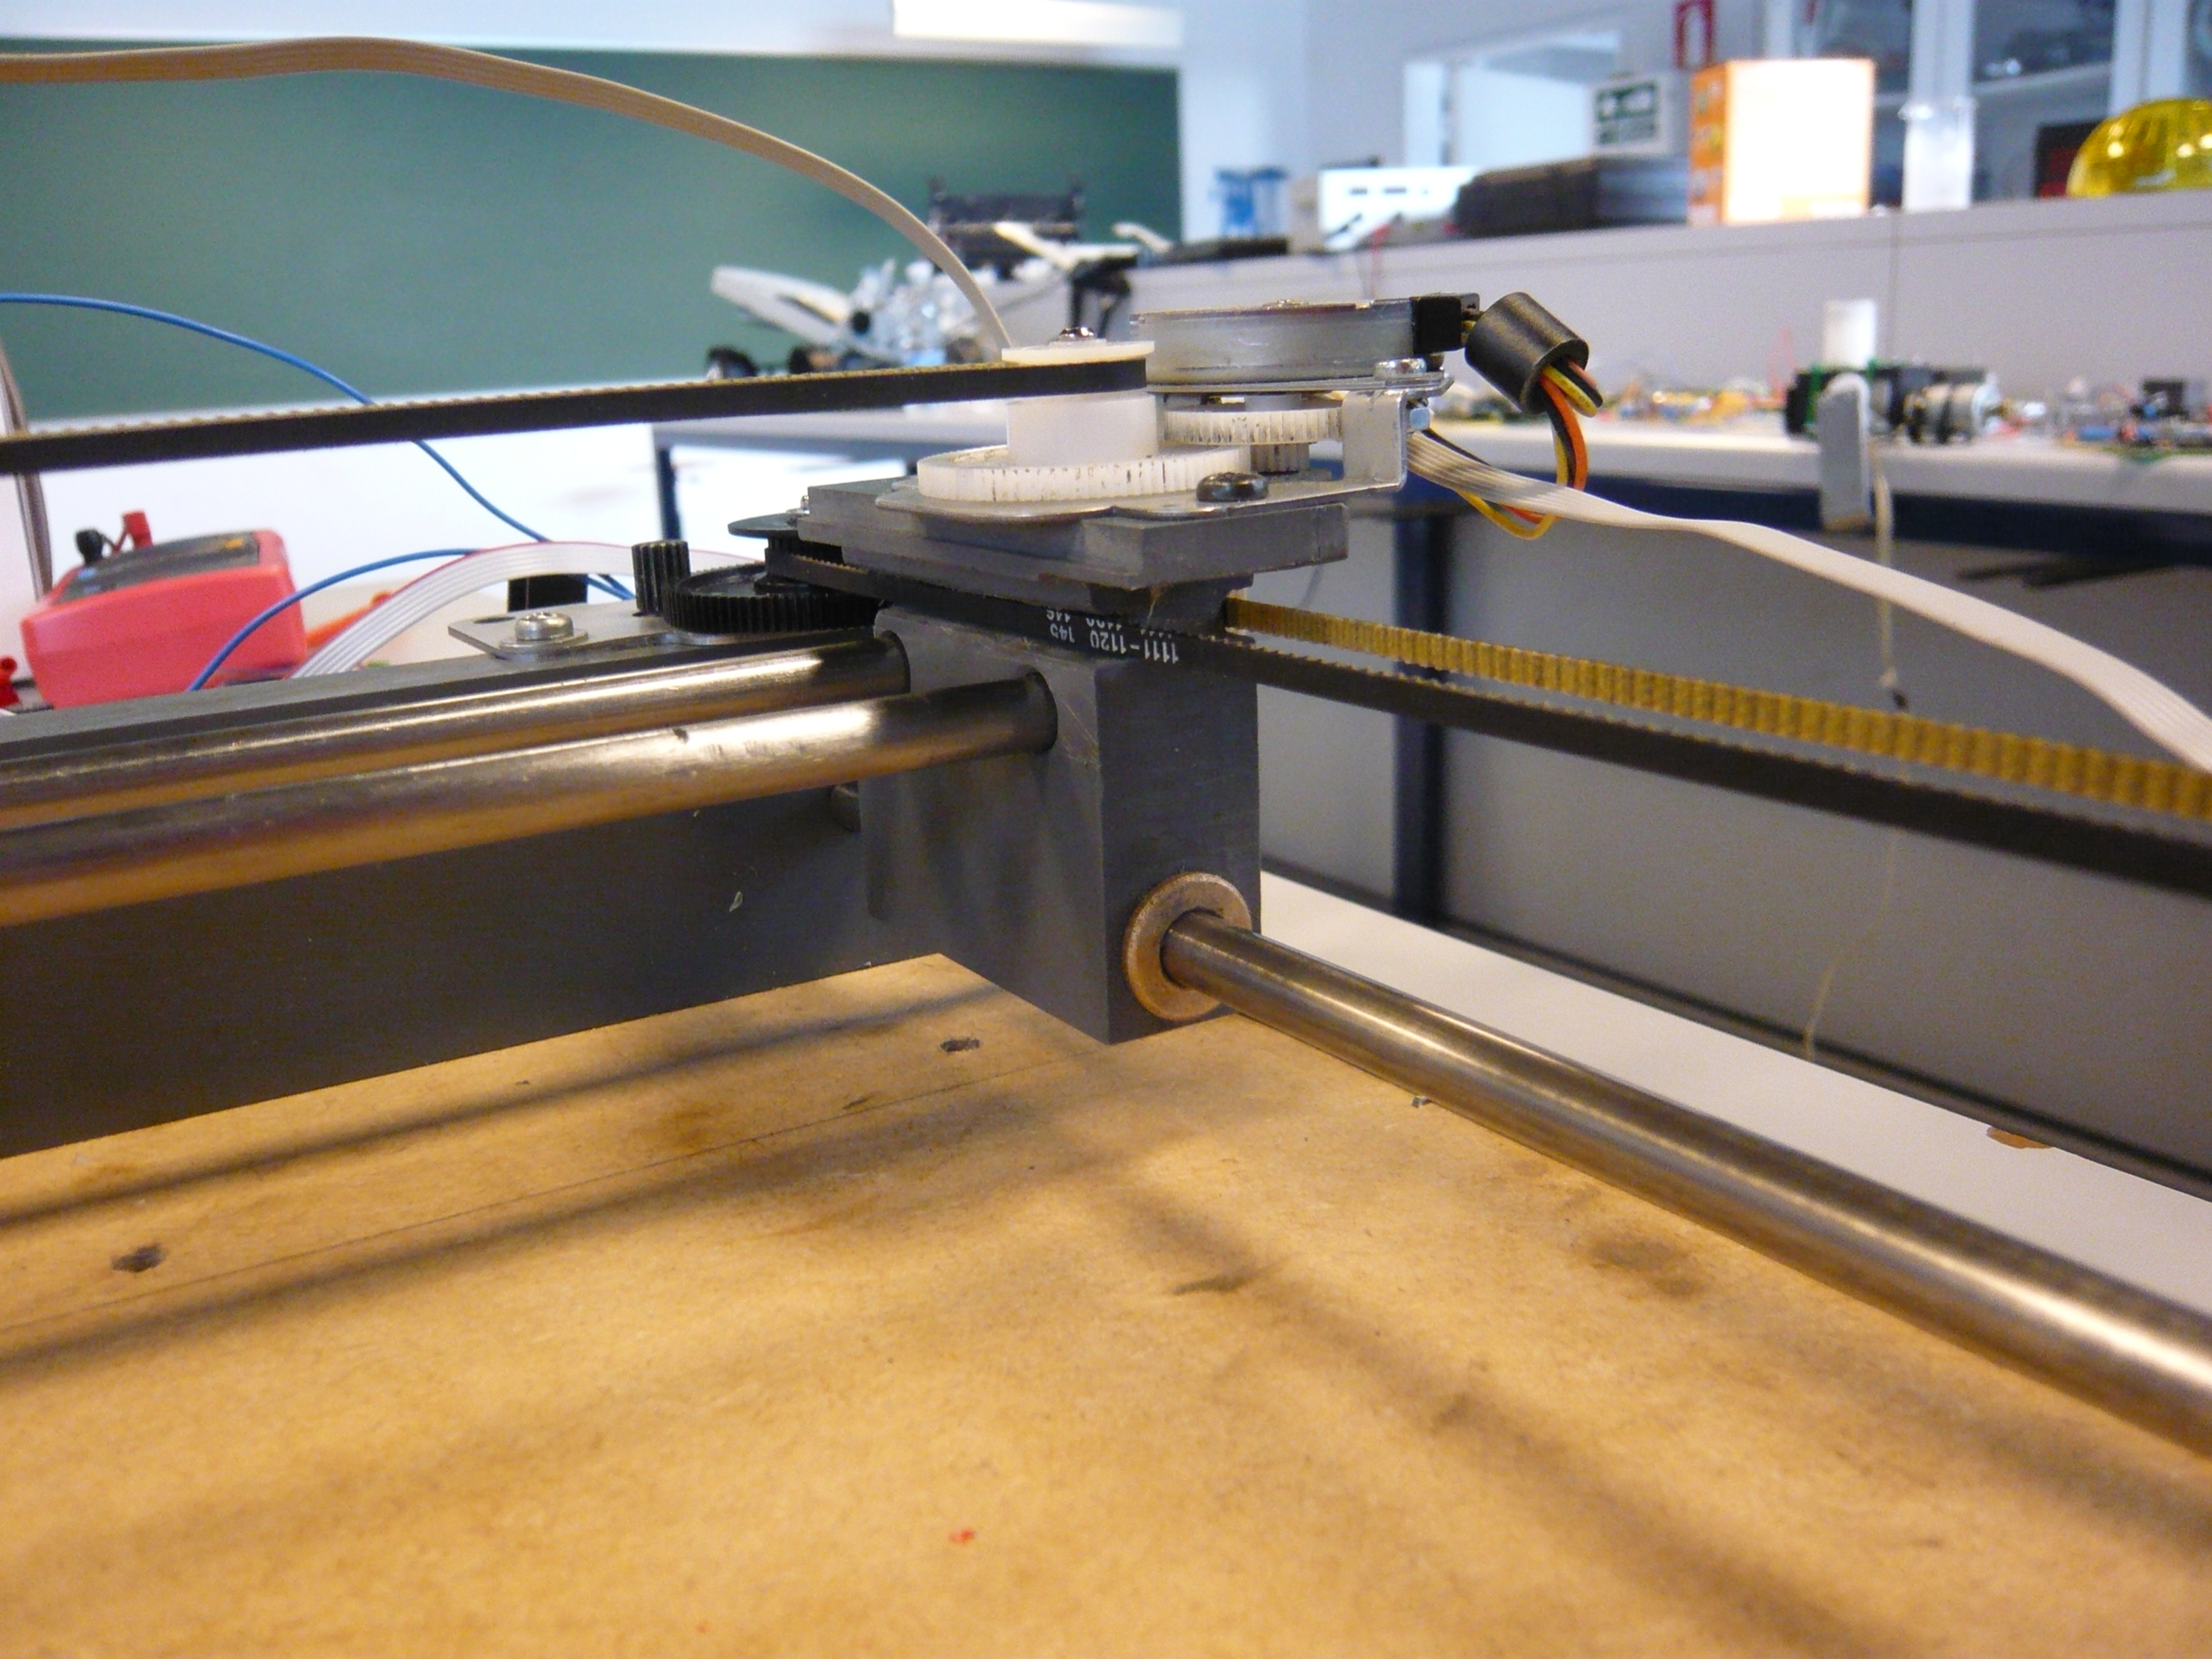
\includegraphics[width=\marginparwidth]{./img/glider}
  \captionof{figure}{Vandret glider}
  \label{fig:glider}
}

Et andet problem omkring slør var placeringen af stepmotoren, som skal
styre gliderne. Her kunne vi placere stepmotoren i midten af selve
konstruktionen eller ude i en af siderne. Hvis
stepmotoren blev placeret i midten af plotteren, så ville det først og
fremmest resultere i en større konstruktion, da stepmotoren skulle
placeres over glideren, men ligeledes ikke gøre meget for at hjælpe på
sløret. Hvis vi istedet placere stepmotoren i siden, som det vises i
afsnit~\vref{sc:stepmotor-driver}, så vil den være i
samme plan som glideren, hvilket ville gøre konstruktionen en del
mindre og samtidig hjælpe på sløret. Glideren ville da først bevæge sig,
når sløret er nogenlunde væk, hvilket giver anledning til en mere
præcis plotning.

Enkelheden af konstruktionen var ligeledes en essentiel del af vores
projekt, da vi har en begrænset periode, hvori vi kan udforme vores
produkt. Produktets størrelser var dog ikke under magen diskusion, da
det simplistiske skulle være en gennemtrængende del uden at have en
indvirkning på produktets funktionalitet. Gliderne samt glidelejrene er
lavet i stål for reduceret gnidningsmodstand. Vi bruger også olie til
yderligere at gøre modstanden mindre, og derved minske sløret.

\fixme{Omformuler dårlige formuleringer} \fixme{Billede med
  betegnelser med de forskellige komponenter på plotteren (tegnehoved,
  glider osv.)}

%%% Local Variables: 
%%% mode: latex
%%% TeX-master: "../master"
%%% End: 